%----------------------------------------------------------------------------------------
%    PACKAGES AND THEMES
%----------------------------------------------------------------------------------------

\documentclass[aspectratio=169,xcolor=dvipsnames]{beamer}
\setbeameroption{show notes} %TODO: Thomas a enlever avant la presentation
\usetheme{SimplePlus}

\usepackage{comment}
\usepackage{hyperref}
\usepackage{graphicx} % Allows including images
\usepackage{booktabs} % Allows the use of \toprule, \midrule and \bottomrule in tables
\usepackage{array} % Allows >{\centering\arraybackslash} in tabular

%----------------------------------------------------------------------------------------
%    TITLE PAGE
%----------------------------------------------------------------------------------------

\title{Stochastic Optimal Control Matching}
\subtitle{Carles Domingo-Enrich, Jiequn Han, Brandon Amos, Joan Bruna, Ricky T. Q. Chen}

\author{Thomas Mousseau}

% \institute
% {
%     Department of Computer Science and Information Engineering \\
%     National Taiwan University % Your institution for the title page
% }
\date{\today} % Date, can be changed to a custom date

%----------------------------------------------------------------------------------------
%    PRESENTATION SLIDES
%----------------------------------------------------------------------------------------

\begin{document}

\begin{frame}
    % Print the title page as the first slide
    \titlepage
\end{frame}

\begin{frame}{Overview}
    % Throughout your presentation, if you choose to use \section{} and \subsection{} commands, these will automatically be printed on this slide as an overview of your presentation
    \tableofcontents
\end{frame}

%------------------------------------------------
\section{Setup and Preliminaries}

\begin{frame}{Evolution of Generative Models}
    \begin{center}
        \begin{minipage}{0.9\textwidth}
            \vspace{0.3cm}
            
            \small
            \begin{tabular}{@{}l@{\hspace{0.8cm}}p{0.75\textwidth}@{}}
                \textbf{2020} & \textbf{DDPM:} Denoising Diffusion Probabilistic Models interpret generation as reversing a discrete noise-adding process, learning to denoise at each step. They produced high-quality samples but required thousands of slow sampling steps. \\[0.4cm]
                
                \textbf{2021} & \textbf{Score-based Models:} Score-based generative models extended diffusion to continuous-time SDEs, learning the score function ($\nabla_x \log p_t(x)$) to reverse a stochastic diffusion process. This unified diffusion with stochastic control, allowed probability flow ODEs, and sped up sampling. \\[0.4cm]
                
                \textbf{2023} & \textbf{Flow Matching:} Flow matching views generation as learning a deterministic ODE vector field that directly transports a simple distribution (e.g., Gaussian) to data. This removed stochasticity and significantly improved efficiency compared to diffusion/score methods. \\[0.4cm]
            \end{tabular}
            
            \vspace{0.3cm}
        \end{minipage}
    \end{center}
\end{frame}

\begin{frame}{SOC as the Foundation of Generative Models}
    \vspace{-0.3cm}
    \begin{block}{The Core Challenge: Unnormalized Densities}
        Generative models must sample from complex distributions $p_{\text{data}}(x) = \frac{1}{Z} \tilde{p}_{\text{data}}(x)$ where the normalization constant $Z = \int \tilde{p}_{\text{data}}(x) dx$ is intractable to compute. This intractability arises from the curse of dimensionality when integrating over high-dimensional spaces.
    \end{block}

    \vspace{-0.3cm}

    \begin{columns}[t]
        \column{0.48\textwidth}
        \begin{alertblock}{SOC Connection}
            \small
            \textbf{Key Insight:} \\
            Transform tractable distributions (Gaussian) to complex target distributions through \textcolor{blue}{optimal control policies}.
            
            \vspace{0.3cm}
            
            This bridges the gap between:
            \begin{itemize}
                \item Simple sampling (easy)
                \item Complex data distributions (hard)
            \end{itemize}
        \end{alertblock}
        
        \column{0.48\textwidth}
        \begin{block}{Modern Implementations}
            \small
            
            \textbf{Diffusion Models:} \\
            $u_t = -\frac{1}{2}\nabla_x \log p_t(x)$ (denoising)
            
            \vspace{0.2cm}
            \textbf{Score-based Models:} \\
            $u_t = \nabla_x \log p_t(x)$ (score function)
            
            \vspace{0.2cm}
            \textbf{Flow Matching:} \\
            $u_t = \frac{x_1 - x_0}{T-t}$ (deterministic flow)
            
            All learn \textcolor{blue}{optimal control policies} to transport distributions!
        \end{block}
    \end{columns}

    \note{
    \textcolor{blue}{\textbf{Unnormalized Densities:}} The fundamental challenge in generative modeling is sampling from distributions $p(x) = \frac{1}{Z}e^{-E(x)}$ where $Z$ is unknown. SOC provides the mathematical framework to construct sampling procedures. \\
    \vspace{0.1cm}
    \textcolor{orange}{\textbf{Historical Context:}} From Langevin dynamics to modern diffusion models, all major breakthroughs in generative modeling can be understood through the lens of stochastic optimal control theory.
    }
\end{frame}

\begin{frame}{What is a Stochastic Control Problem?}
    
    \begin{block}{Control-Affine Stochastic Differential Equation}
        The general form of a controlled stochastic process:
        \begin{equation}
        dX_t^u = \big(b(X_t^u, t) + \sigma(t)u(X_t^u, t)\big) dt + \sqrt{\lambda}\sigma(t) dB_t
        \end{equation}
    \end{block}

            \vspace{0.3cm}
    
            \textbf{State Process:} $X_t^u \in \mathbb{R}^d$ (system state under control $u$ at time $t$)
            
            \vspace{0.3cm}
            
            \textbf{Drift Term:} $b(X_t^u, t) \in \mathbb{R}^d$ (natural evolution of the system)
            
            \vspace{0.3cm}
            
            \textbf{Control Term:} $\sigma(t)u(X_t^u, t) \in \mathbb{R}^d$ (how control influences the system)
            
            \vspace{0.3cm}
            
            \textbf{Diffusion Coefficient:} $\sigma(t) \in \mathbb{R}^{d \times d}$ (volatility matrix)
            
            \vspace{0.3cm}
            
            \textbf{Noise Process:} $B_t \in \mathbb{R}^d$ (Brownian motion, external randomness)
            
            \vspace{0.3cm}
            
            \textbf{Noise Intensity:} $\lambda > 0$ (controls the strength of stochastic perturbations)

    \note{
    \textcolor{blue}{\textbf{Control-Affine Structure:}} The "control-affine" property means the control $u$ enters linearly (affinely) in the drift term. This is the most general practical form for controlled SDEs, encompassing most applications in finance, robotics, and machine learning. \\    
    \vspace{0.1cm}

   \textcolor{red}{Je dois aussi expliquer l'importance que le steering input ainsi que le noise sont tous les 2 multipliés par sigma(t) ce qui signifie que ...}
    }
\end{frame}

\begin{frame}{The Optimal Control Objective}
    \vspace{-0.3cm}
    
    \begin{block}{Cost Function to Minimize}
        Find the optimal control policy $u^* \in \mathcal{U}$ that minimizes:
        \begin{equation}
        \min_{u \in \mathcal{U}} \mathbb{E}\left[\int_0^T \left(\frac{1}{2}\|u(X_t^u, t)\|^2 + f(X_t^u, t)\right) dt + g(X_T^u)\right]
        \end{equation}
    \end{block}

            \vspace{0.3cm}
    
             \textbf{Control Effort:} $\frac{1}{2}\|u(X_t^u, t)\|^2$ (penalizes large control actions)

            \vspace{0.3cm}

             \textbf{Running Cost:} $f(X_t^u, t)$ (ongoing cost during the process evolution)

            \vspace{0.3cm}

             \textbf{Terminal Cost:} $g(X_T^u)$ (final cost based on end state at time $T$)
            
            \vspace{0.3cm}
            
             \textbf{Control Space:} $\mathcal{U}$ (set of admissible control policies)

    \note{

    }
    
\end{frame}

\begin{frame}{SOC in Practice}

    \vspace{-0.3cm}
    \begin{table}
        \centering
        \small
        \begin{tabular}{>{\centering\arraybackslash}p{0.25\textwidth}|>{\centering\arraybackslash}p{0.22\textwidth}|>{\centering\arraybackslash}p{0.22\textwidth}|>{\centering\arraybackslash}p{0.22\textwidth}}
            \toprule
            \textbf{Aspect} & \textbf{Steering Actuator} & \textbf{Diffusion Models} & \textbf{Flow Models} \\
            \midrule
            \textbf{State $X_t$} & Vehicle position, velocity & Noisy data sample & Clean data sample \\
            \midrule
            \textbf{Control $u_t$} & Steering angle, throttle & Denoising direction & Flow velocity field \\
            \midrule
            \textbf{Dynamics Source} & \textcolor{blue}{Newtonian mechanics} (vehicle dynamics) & \textcolor{orange}{Forward noising} process & \textcolor{ForestGreen}{No natural drift} (learnable) \\
            \midrule
            \textbf{Drift $b(X_t,t)$} & Kinematic equations & Predetermined schedule & $b = 0$ (control learns drift) \\
            \midrule
            \textbf{Control Goal} & Reach target safely & Reverse noise process & Transport distributions \\
            \midrule
            \textbf{Noise $\sqrt{\lambda}\sigma dB_t$} & Road disturbances & Brownian motion & Optional stochasticity \\
            \bottomrule
        \end{tabular}
    \end{table}
    
    \vspace{0.3cm}
    
    \begin{alertblock}{Key Insight}
        \textbf{Same mathematical framework, different physics:} SOC unifies vehicle control, generative modeling, and distribution transport under a single theoretical umbrella.
    \end{alertblock}

    \note{
    \textcolor{blue}{\textbf{Steering Actuator:}} The dynamics come from well-established physics - Newton's laws, kinematics, and vehicle dynamics. The control optimizes safety and efficiency. \\
    \vspace{0.1cm}
    \textcolor{orange}{\textbf{Diffusion Models:}} The drift is determined by the forward noising process (e.g., $\beta(t)$), and control learns to reverse this predetermined corruption. \\
    \vspace{0.1cm}
    \textcolor{ForestGreen}{\textbf{Flow Models:}} No natural drift exists - the control $u_t$ directly becomes the drift term, learning the entire velocity field that transports distributions.
    }
\end{frame}


\begin{comment}
\begin{frame}{Classic Approach to Finding Optimal Control}
    \begin{block}{Optimal Control $u^*$}
        Find the control policy $u^*$ that minimizes the expected cost: $u^* = \arg\min_u J(u)$
    \end{block}
        
    \begin{block}{Hamilton-Jacobi-Bellman (HJB) Equation}
        The classical approach uses the HJB PDE to characterize the value function $V(x,t)$:
        \small
        \begin{equation}
        \frac{\partial V}{\partial t} + \min_u \left[ L(x,u,t) + \frac{\partial V}{\partial x} f(x,u,t) + \frac{1}{2}\text{tr}(\sigma^T \nabla^2 V \sigma) \right] = 0
        \end{equation}
        
        \vspace{0.2cm}
        With boundary condition: $V(x,T) = \Phi(x)$ (terminal cost)
    \end{block}
        
    \begin{alertblock}{The Curse of Dimensionality}
        Classical numerical methods (finite differences, grid-based) become \textcolor{red}{computationally intractable} in high dimensions due to exponential growth in grid size: $\mathcal{O}(N^d)$ where $d$ is dimension.
    \end{alertblock}

    \note{
    \textcolor{blue}{\textbf{HJB Equation:}} The Hamilton-Jacobi-Bellman equation provides the theoretical foundation for solving stochastic optimal control problems by characterizing the value function $V(x,t)$ as the solution to a nonlinear PDE. The optimal control is then $u^*(x,t) = \arg\min_u [\cdots]$ from the HJB equation.
    }
\end{frame}
\end{comment}

\begin{comment}
\begin{frame}{Neural PDE Solvers for SOC}
    
    \begin{block}{Core Innovation: Neural ODEs (Chen et al., 2018)}
        \textcolor{blue}{\textbf{Key Insight:}} Replace discrete layers with continuous-time ODEs \\
        $\frac{dh(t)}{dt} = f_\theta(h(t), t)$ where $h(t)$ represents hidden states evolving continuously
    \end{block}

    \vspace{-0.3cm}

    \begin{columns}[t]
        \column{0.48\textwidth}
        \begin{alertblock}{Neural Network Approximation}
            \small
            \textbf{Value Function:}
            \begin{equation}
            V(x,t) \approx V_\theta(x,t)
            \end{equation}
            
            \textbf{Control Policy:}
            \begin{equation}
            u(x,t) \approx u_\phi(x,t)
            \end{equation}
            
            Both parameterized by deep neural networks
        \end{alertblock}
        
        \column{0.48\textwidth}
        \begin{block}{Training Process}
            \small
            \textbf{Physics-Informed Loss:}
            \begin{equation}
            \mathcal{L} = \|HJB_{residual}\|^2 + \|BC_{error}\|^2
            \end{equation}
            
            \textbf{Key Components:}
            \begin{itemize}
                \item \textcolor{blue}{Automatic differentiation} for PDE terms
                \item \textcolor{ForestGreen}{Adjoint method} for gradients
                \item \textcolor{orange}{Stochastic sampling} of $(x,t)$ points
            \end{itemize}
        \end{block}
    \end{columns}
    
    \vspace{0.3cm}
    
    \begin{block}{Advantages Over Classical Methods}
        \begin{itemize}
            \item \textcolor{ForestGreen}{\textbf{High-dimensional scalability:}} No curse of dimensionality
            \item \textcolor{ForestGreen}{\textbf{Mesh-free:}} No spatial discretization required  
            \item \textcolor{orange}{\textbf{Limitation:}} Requires careful tuning and may lack convergence guarantees
        \end{itemize}
    \end{block}

    \note{
    \textcolor{blue}{\textbf{Neural ODEs:}} Chen et al. (2018) showed that residual networks can be interpreted as discretizations of ODEs. This insight led to continuous-depth models and, crucially for our context, neural methods for solving differential equations. \\
    \vspace{0.1cm}
    \textcolor{ForestGreen}{\textbf{Physics-Informed Neural Networks:}} The key is training networks to satisfy the HJB equation through the residual loss, making the physics constraints part of the optimization objective.
    }
\end{frame}
\end{comment}

%------------------------------------------------
\section{Stochastic Optimal Control Matching}

\begin{frame}{Applications of SOC}
    
    \begin{block}{Key ML Applications of SOC}
        \begin{itemize}
            \item \textbf{Reward fine-tuning of diffusion and flow models:} Optimizing generation quality using reward signals
            
            \vspace{0.2cm}
            
            \item \textbf{Conditional sampling on diffusion and flow models:} Steering generation towards specific conditions or constraints
            
            \vspace{0.2cm}
            
            \item \textbf{Sampling from unnormalized densities:} Efficiently drawing samples from complex, intractable distributions
            
            \vspace{0.2cm}
            
            \item \textbf{Importance sampling of rare events in SDEs:} Computing probabilities of low-probability but critical events
        \end{itemize}
    \end{block}

    \vspace{-0.1cm}
    
    \begin{alertblock}{Key Insight}
        The prevalence of SOC formulations in modern ML motivates the need for more efficient and stable solving methods.
    \end{alertblock}

    \note{\textcolor{red}{Je dois etre capable de vraiment bien expliquer les applications du SOC dans le ML moderne pour pouvoir demontrer l'importance d'avoir pris ce papier}}
\end{frame}

\begin{frame}{Solve SOC Problems in Low Dimension}
    \vspace{-0.1cm}
    
    \begin{block}{Classical Approach: Hamilton-Jacobi-Bellman PDE}
        In small state spaces (1D, 2D, sometimes 3D), discretize the state space and solve the HJB PDE directly:
        \begin{equation}
        \frac{\partial V}{\partial t} + \min_u \left[ \frac{1}{2}\|u\|^2 + f(x,t) + \nabla V \cdot (b + \sigma u) + \frac{1}{2}\lambda \text{tr}(\sigma^T \nabla^2 V \sigma) \right] = 0
        \end{equation}
    \end{block}

    \vspace{-0.4cm}
    
    \begin{columns}[t]
        \column{0.48\textwidth}
        \begin{block}{What You Get}
            \begin{itemize}
                \item \textcolor{ForestGreen}{\textbf{Value function:}} $V(x,t)$
                \item \textcolor{ForestGreen}{\textbf{Optimal control:}} $u^*(x,t) = -\sigma(t)^T \nabla V(x,t)$
                \item \textcolor{ForestGreen}{\textbf{Global optimum}} guaranteed
                \item \textcolor{ForestGreen}{\textbf{Theoretical guarantees}} (convergence, stability)
            \end{itemize}
        \end{block}
        
        \column{0.48\textwidth}
        \begin{alertblock}{The Curse of Dimensionality}
            \begin{itemize}
                \item \textcolor{red}{\textbf{Grid size:}} $\mathcal{O}(N^d)$ where $d$ is dimension
                \item \textcolor{red}{\textbf{Memory:}} Exponential growth with $d$
                \item \textcolor{red}{\textbf{Computation:}} Infeasible for $d > 3$
                \item \textcolor{red}{\textbf{Impossible}} to discretize for $d \gg 1$
            \end{itemize}
        \end{alertblock}
    \end{columns}


    \note{
        \textbf{Works perfectly in low dimensions, but state space grows exponentially with dimension.}

    \textcolor{blue}{\textbf{Classical HJB:}} In low dimensions, you can discretize the entire state space on a grid and solve the HJB PDE using finite difference methods. This gives you the exact solution but becomes computationally impossible as dimension increases. \\
    \vspace{0.1cm}
    \textcolor{red}{\textbf{Curse of Dimensionality:}} For a $d$-dimensional problem with $N$ grid points per dimension, you need $N^d$ total grid points. Even modest problems ($d=10$, $N=100$) require $100^{10} = 10^{20}$ grid points.
    }
\end{frame}

\begin{frame}{Solve SOC Problems in High Dimension}
    \vspace{-0.1cm}
    
    \begin{block}{Modern Approach: Adjoint Methods}
        Cannot discretize high-dimensional spaces, so use \textcolor{blue}{\textbf{adjoint methods}} to optimize control directly:
        \begin{equation}
        \min_{u} \mathbb{E}\left[\int_0^T \left(\frac{1}{2}\|u(X_t^u, t)\|^2 + f(X_t^u, t)\right) dt + g(X_T^u)\right]
        \end{equation}
    \end{block}

    \vspace{-0.4cm}

    \begin{columns}[t]
        \column{0.48\textwidth}
        \begin{block}{What You Get}
            \begin{itemize}
                \item \textcolor{ForestGreen}{\textbf{Scalable:}} Works in high dimensions
                \item \textcolor{ForestGreen}{\textbf{Neural networks:}} Can parameterize complex controls
                \item \textcolor{ForestGreen}{\textbf{Gradient-based:}} Standard optimization techniques
            \end{itemize}
        \end{block}
        
        \column{0.48\textwidth}
        \begin{alertblock}{Major Problem}
            \begin{itemize}
                \item \textcolor{red}{\textbf{Non-convex landscape:}} Full of local minima
                \item \textcolor{red}{\textbf{Unstable training:}} Difficult optimization
                \item \textcolor{red}{\textbf{No guarantees:}} May not find global optimum
                \item \textcolor{red}{\textbf{Sensitive initialization:}} Results vary significantly
            \end{itemize}
        \end{alertblock}
    \end{columns}
    
    \note{
    \textbf{Highly non-convex functional landscape makes optimization extremely challenging.} \\
    Traditional SOC methods struggle with local minima and unstable training dynamics.

    \vspace{0.1cm}

    \textcolor{blue}{\textbf{Adjoint Methods:}} These methods solve the forward SDE and then use the adjoint equation to compute gradients efficiently. This allows gradient-based optimization of the control parameters without discretizing the state space. \\
    \vspace{0.1cm}
    \textcolor{red}{\textbf{Non-convex Optimization:}} The major challenge is that the resulting optimization landscape is highly non-convex, leading to difficult optimization with many local minima and unstable training dynamics.
    }
\end{frame}

\begin{frame}{Similar Trend in Generative Modeling}
    \vspace{-0.1cm}
    
    \begin{block}{The Same Pattern: Non-convex → Least-Squares}
        Generative modeling experienced the same transition from non-convex to convex optimization
    \end{block}
        
    \vspace{-0.4cm}

    \begin{columns}[t]
        \column{0.48\textwidth}
        \begin{alertblock}{Continuous Normalizing Flows}
            \small
            \textbf{Method:} Learn invertible transformations
            \begin{equation}
            \frac{dx}{dt} = f_\theta(x, t)
            \end{equation}
            
            \textbf{Problem:}
            \begin{itemize}
                \item Use \textcolor{red}{\textbf{adjoint methods}} for gradients
                \item \textcolor{red}{\textbf{Non-convex}} optimization landscape
                \item Difficult training, unstable dynamics
            \end{itemize}
        \end{alertblock}
        
        \column{0.48\textwidth}
        \begin{block}{Denoising Diffusion Models}
            \small
            \textbf{Method:} Learn to reverse noise process
            \begin{equation}
            \mathbb{E}[\|\epsilon_\theta(x_t, t) - \epsilon\|^2]
            \end{equation}
            
            \textbf{Advantage:}
            \begin{itemize}
                \item Use \textcolor{ForestGreen}{\textbf{least-squares loss}} 
                \item \textcolor{ForestGreen}{\textbf{Convex}} functional landscape
                \item Stable, reliable optimization
            \end{itemize}
        \end{block}
    \end{columns}
        
    \note{
    \textbf{Insight:} Apply the same principle to SOC! Replace non-convex adjoint methods with \textcolor{blue}{\textbf{least-squares matching}}, creating a \textcolor{ForestGreen}{\textbf{convex optimization landscape}} for stochastic optimal control.
    \\
    \vspace{0.1cm}
    \textcolor{orange}{\textbf{Historical Parallel:}} Continuous Normalizing Flows (CNFs) suffered from the same optimization challenges as traditional SOC - they used adjoint methods and had non-convex landscapes. DDPMs revolutionized generative modeling by reformulating the problem as least-squares regression. \\
    \vspace{0.1cm}
    \textcolor{blue}{\textbf{SOCM's Contribution:}} SOCM brings the same insight to stochastic optimal control, replacing direct optimization with least-squares matching to achieve stable, convex optimization.
    }
\end{frame}

\begin{comment}
\begin{frame}{Reasons behind SOCM (2/2)}
    Current SOC methods suffer from optimization challenges that limit their effectiveness.
    
    \vspace{0.3cm}
    
    \begin{columns}[t]
        \column{0.48\textwidth}
        \begin{alertblock}{Current SOC Methods}
            \begin{itemize}
                \item Use \textbf{adjoint methods} (like CNFs)
                \item Yield \textbf{non-convex} function landscapes
                \item Difficult optimization with local minima
                \item Unstable training dynamics
            \end{itemize}
        \end{alertblock}
        
        \column{0.48\textwidth}
        \begin{block}{Diffusion Models Success}
            \begin{itemize}
                \item Use \textbf{least-squares loss}
                \item Create \textbf{convex} functional landscapes
                \item Stable and reliable optimization
                \item Excellent empirical performance
            \end{itemize}
        \end{block}
    \end{columns}
    
    \vspace{0.4cm}
    
    \begin{block}{SOCM's Innovation}
        \textbf{Goal:} Develop least-squares loss formulations for SOC problems, combining the expressiveness of stochastic control with the optimization stability of diffusion models.
    \end{block}
\end{frame}
\end{comment}


\begin{frame}{SOCM in Context: Optimization Landscapes}
    \vspace{0.5cm}
    \begin{table}
        \centering
        \begin{tabular}{>{\centering\arraybackslash}p{0.25\textwidth}>{\centering\arraybackslash}p{0.35\textwidth}>{\centering\arraybackslash}p{0.35\textwidth}}
            \toprule
            \textbf{Task} & \textbf{Non-convex} & \textbf{Least Squares} \\
            \midrule
            Generative Modeling & Maximum Likelihood CNFs & Diffusion models and Flow Matching \\
            Stochastic Optimal Control & Adjoint Methods & \textcolor{red}{\textbf{Stochastic Optimal Control Matching}} \\
            \bottomrule
        \end{tabular}
    \end{table}
\end{frame}

\begin{comment}
\begin{frame}{Introducing Stochastic Optimal Control Matching}
    SOCM offers a more principled, stable, and accurate way to learn generative dynamics by blending stochastic control theory with modern matching-based generative modeling.
    
    \vspace{0.4cm}
    
    \begin{block}{Key Novel Contributions}
        \begin{enumerate}
            \item \textbf{Controlled Stochastic Process:} Views the generation process as a controlled stochastic process bridging a simple distribution to data.
            
            \vspace{0.2cm}
            
            \item \textbf{Least-Squares Matching:} Learning the control via least-squares matching, a stable and convex regression objective.
            
            \vspace{0.2cm}
            
            \item \textbf{Joint Optimization:} Optimizing control and variance-reducing reparameterization matrices simultaneously, for efficient learning.
            
            \vspace{0.2cm}
            
            \item \textbf{Path-wise Reparameterization:} Introducing a path-wise reparameterization trick, boosting gradient estimation quality.
        \end{enumerate}
    \end{block}
\end{frame}
\end{comment}

\begin{frame}{SOCM Framework: From Classical SOC to SOCM}
    \small
    \begin{block}{Dynamics (Same for Both)}
        \begin{equation}
        dX^v_t = (b(X^v_t, t) + \sigma(t)v(X^v_t, t)) dt + \sqrt{\lambda}\sigma(t) dB_t \text{, with } X^v_0 \sim p_0
        \end{equation}
    \end{block}

    \begin{block}{Original SOC Cost Function}
        \begin{equation}
        \min_{u \in \mathcal{U}} \mathcal{L}_{SOC} := \mathbb{E}\left[\int_0^T \left(\frac{1}{2}\|u(X_t^u, t)\|^2 + f(X_t^u, t)\right) dt + g(X_T^u)\right]
        \end{equation}
    \end{block}

    \begin{alertblock}{SOCM Cost Function}
        \begin{equation}
        \min_{u, M} \mathcal{L}_{SOCM}(u, M) := \mathbb{E}\left[\frac{1}{T}\int_0^T \|u(X^v_t, t) - w(t, v, X^v, B, M_t)\|^2 dt \times \alpha(v, X^v, B)\right]
        \end{equation}
    \end{alertblock}

    \vspace{0.2cm}
    \small
    \textbf{Key Point:} Same underlying stochastic dynamics, but SOCM uses a \textcolor{blue}{least-squares matching approach} instead of direct minimization of the original cost.
\end{frame}

\begin{frame}{SOCM Parameters Definition}
    
    $$\min_{\textcolor{blue}{u}, \textcolor{red}{M}} \mathcal{L}_{SOCM}(\textcolor{blue}{u}, \textcolor{red}{M}) := \mathbb{E}\left[\frac{1}{T}\int_0^T \|\textcolor{blue}{u}(X^{\textcolor{orange}{v}}_t, t) - \textcolor{ForestGreen}{w}(t, \textcolor{orange}{v}, X^{\textcolor{orange}{v}}, B, \textcolor{red}{M_t})\|^2 dt \times \textcolor{purple}{\alpha}(\textcolor{orange}{v}, X^{\textcolor{orange}{v}}, B)\right]$$
        
    \begin{block}{Where:}
            $u : \mathbb{R}^d \times [0,1] \rightarrow \mathbb{R}^d$ is the \textcolor{blue}{\textbf{control}} (policy being learned)
            \vspace{0.1cm} \\
            $v$ is a \textcolor{orange}{\textbf{fixed arbitrary control}}, $X^v$ is the solution of the SDE with control $v$
            \vspace{0.1cm} \\
            $M : [0,1]^2 \rightarrow \mathbb{R}^{d \times d}$ is the \textcolor{red}{\textbf{reparameterization matrix}}
            \vspace{0.1cm} \\
            $w$ is the \textcolor{ForestGreen}{\textbf{matching vector field}} (target for $u$ to match)
            \vspace{0.1cm} \\
            $\alpha$ is the \textcolor{purple}{\textbf{importance weight}} (for measure correction)
    \end{block}
        
    \begin{alertblock}{Key Dependencies}
        $w$ and $\alpha$ depend on $f$, $g$, $\lambda$, $\sigma$
    \end{alertblock}

    \note{
    \textcolor{blue}{\textbf{Control $u$:}} This is what we're trying to learn - the optimal policy that minimizes our cost function. \\
    \vspace{0.1cm}
    \textcolor{orange}{\textbf{Arbitrary Control $v$:}} Used to generate sample trajectories for training. The choice of $v$ affects the efficiency but not the correctness of SOCM. \\
    \vspace{0.1cm}
    \textcolor{red}{\textbf{Reparameterization Matrix $M$:}} Jointly optimized with $u$ to reduce variance in the gradient estimation through path-wise reparameterization.
    }
\end{frame}



\begin{frame}{Matching Vector Field (1/2)}
    \vspace{-0.3cm}
    
    \begin{block}{Reparameterization Function $w(t, v, X^v, B, M_t)$}
        \small
        The \textcolor{blue}{\textbf{matching vector field}} computed via path-wise reparameterization:
        \vspace{-0.2cm}
        \begin{equation}
        \begin{aligned}
        w(t, v, X^v, B, M_t) 
        = \sigma(t)^\top \Bigg(
        &- \int_t^T M_t(s) \nabla_x f(X_s^v, s)\, ds 
           \;-\; M_t(T)\nabla g(X_T^v) \\[4pt]
        &+ \int_t^T \big(M_t(s)\nabla_x b(X_s^v, s) - \partial_s M_t(s)\big)(\sigma^{-1}(s))^\top v(X_s^v, s)\, ds \\[4pt]
        &+ \sqrt{\lambda} \int_t^T \big(M_t(s)\nabla_x b(X_s^v, s) - \partial_s M_t(s)\big)(\sigma^{-1}(s))^\top dB_s
        \Bigg)
        \end{aligned}
        \end{equation}
        
        Where $M_t(s)$ is the \textcolor{ForestGreen}{\textbf{reparameterization matrix}} (learned jointly with $u$)
    \end{block}

\end{frame}

\begin{frame}[allowframebreaks]{Matching Vector Field (2/2) - Derivation Steps}
    \vspace{-0.3cm}
    
    % Make section titles more prominent
    \begin{center}
        \Large\textcolor{blue}{\textbf{Step 1 — Path-integral form of $u^*$ (Kappen 2005)}}
    \end{center}
    
    \vspace{0.3cm}
    
    \begin{block}{What to Show}
        We want to eliminate the value function $V$ from the optimal control formula and express $u^*$ directly in terms of path integrals.
    \end{block}
    
    \vspace{0.5cm}
    
    \subsection*{Starting Point: Value Function Definition}
    
    The value function is defined as the infimum over all controls:
    $$V(x,t) = \inf_u J(u; x,t) = \inf_u \mathbb{E}\left[\int_t^T \left(\frac{1}{2}\|u\|^2 + f\right) ds + g(X_T) \,\middle|\, X_t = x\right]$$
    
    \vspace{0.5cm}
    
    \subsection*{Infinitesimal Generator and HJB Equation}
    
    The \textcolor{blue}{\textbf{infinitesimal generator}} $L$ of the uncontrolled diffusion $dX_t = b \, dt + \sqrt{\lambda} \sigma \, dB_t$ is:
    $$L = b \cdot \nabla + \frac{\lambda}{2} \text{tr}(\sigma \sigma^T \nabla^2)$$
    
    The Hamilton-Jacobi-Bellman equation becomes:
    $$\frac{\partial V}{\partial t} + LV + \inf_u \left[\frac{1}{2}\|u\|^2 + f + u^T \sigma^T \nabla V\right] = 0$$
    
    \vspace{0.5cm}
    
    \subsection*{Deriving the Optimal Control}
    
    To find the infimum, we differentiate the expression inside the brackets with respect to $u$:
    $$\frac{\partial}{\partial u}\left[\frac{1}{2}\|u\|^2 + u^T \sigma^T \nabla V\right] = u + \sigma^T \nabla V = 0$$
    
    This gives us the \textcolor{red}{\textbf{optimal control}}:
    $$u^*(x,t) = -\sigma^T(t)\nabla V(x,t)$$
    
    Substituting back into the HJB equation:
    $$\frac{\partial V}{\partial t} + LV - \frac{1}{2}\|\sigma^T \nabla V\|^2 + f = 0, \quad V(x,T) = g(x)$$
    
    \vspace{0.8cm}
    
    \subsection*{Key Insight: Path-integral Value Function}
    
    For the \textcolor{blue}{\textbf{uncontrolled SDE}} $dX_t = b \, dt + \sqrt{\lambda} \sigma \, dB_t$, the value function has a path-integral representation:
    
    $$V(x,t) = -\lambda \log \mathbb{E}\left[\exp\left(-\frac{1}{\lambda}\int_t^T f(X_s,s) ds - \frac{1}{\lambda} g(X_T)\right) \,\middle|\, X_t = x\right]$$
    
    \vspace{0.8cm}
    
    \subsection*{Result: Lemma 1}
    
    Combining the optimal control formula with the path-integral representation:
    
    \begin{alertblock}{Path-integral Optimal Control}
        $$u^*(x,t) = \lambda \, \sigma^T(t) \, \nabla_x \log \mathbb{E}\left[\exp\left(-\frac{1}{\lambda}\int_t^T f(X_s,s) ds - \frac{1}{\lambda} g(X_T)\right) \,\middle|\, X_t = x\right]$$
    \end{alertblock}
    
    \vspace{0.8cm}
    
    \begin{block}{Why This Matters}
        \textbf{Key Achievement:} This eliminates $V$ from the formula for $u^*$ and reframes \textcolor{ForestGreen}{\textbf{"learning a control"}} as \textcolor{blue}{\textbf{learning a score}} (a gradient of a log-partition function over paths).
        
        \vspace{0.3cm}
        
        This is exactly the kind of signal we can estimate and match via \textcolor{red}{\textbf{least squares}} — setting up the foundation for SOCM's approach.
    \end{block}
    
    \framebreak
    
    % Step 2 on next frame break
    \begin{center}
        \Large\textcolor{red}{\textbf{Step 2 — Path-wise Reparameterization Trick}}
    \end{center}
    
    \vspace{0.3cm}
    
    \begin{block}{The Challenge}
        Direct estimation of the path-integral in Step 1 has high variance and is computationally intractable for complex problems.
    \end{block}
    
    % Add Step 2 content here...
    
    \framebreak
    
    % Step 3 on next frame break
    \begin{center}
        \Large\textcolor{ForestGreen}{\textbf{Step 3 — Girsanov Theorem Application}}
    \end{center}
    
    \vspace{0.3cm}
    
    \begin{block}{The Goal}
        Transform the uncontrolled process into a controlled process using measure theory.
    \end{block}
    
    % Add Step 3 content here...

\end{frame}

    
\begin{frame}{Importance Weight (1/2)}
    
    \begin{block}{Importance Weight $\alpha(v, X^v, B)$}
        \small
        The \textcolor{red}{\textbf{importance sampling weight}} for measure correction:
        \vspace{-0.2cm}
        \begin{equation}
        \begin{aligned}
        \alpha(v, X^v, B) = \exp\!\Bigg(
        &- \frac{1}{\lambda}\int_0^T f(X_t^v, t)\, dt
        - \frac{1}{\lambda} g(X_T^v) \\[4pt]
        &- \frac{1}{\sqrt{\lambda}} \int_0^T \langle v(X_t^v, t), dB_t \rangle
        - \frac{1}{2\lambda} \int_0^T \| v(X_t^v, t) \|^2 dt
        \Bigg)
        \end{aligned}
        \end{equation}

        Incorporates \textcolor{orange}{running costs}, \textcolor{orange}{terminal costs}, and \textcolor{orange}{control effort}
    \end{block}

    \note{
    \textcolor{blue}{\textbf{Reparameterization Matrix $M_t$:}} This matrix enables path-wise reparameterization, a technique to reduce variance in gradient estimation by reparameterizing the stochastic process. It's optimized jointly with the control $u$ to minimize the overall SOCM loss. \\
    \vspace{0.1cm}
    \textcolor{red}{\textbf{Importance Weight $\alpha$:}} This exponential weight corrects for the mismatch between the learned control measure and the optimal control measure. However, it can have high variance when costs are large or in high dimensions, which is the main limitation of SOCM.
    }
\end{frame}


\begin{frame}{SOCM Algorithm}
    \begin{figure}
        \centering
        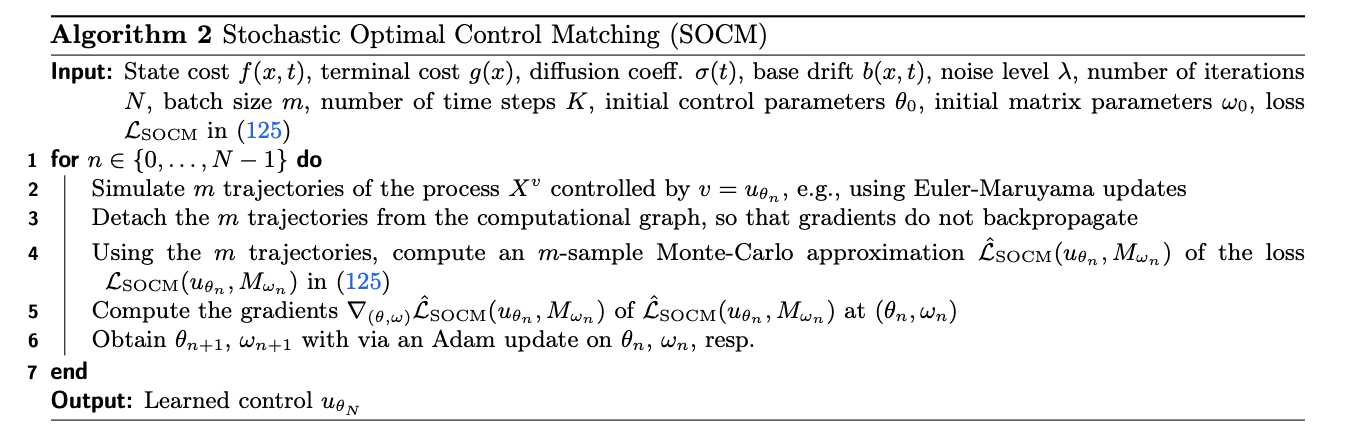
\includegraphics[width=0.95\textwidth]{figures/SOCM_algo.png}
        \caption{Stochastic Optimal Control Matching (SOCM) Algorithm}
    \end{figure}
\end{frame}

%------------------------------------------------

%------------------------------------------------

\section{Experiments and results}

\begin{frame}{Ornstein Uhlenbeck Process}
    \begin{block}{Definition}
        The Ornstein-Uhlenbeck process is a stochastic process that describes the evolution of a variable over time, incorporating both deterministic and stochastic elements. It is often used to model mean-reverting behavior in financial markets and other systems.
    \end{block}
\end{frame}

\begin{frame}{Experimental Results (1/2)}
    \begin{figure}
        \centering
        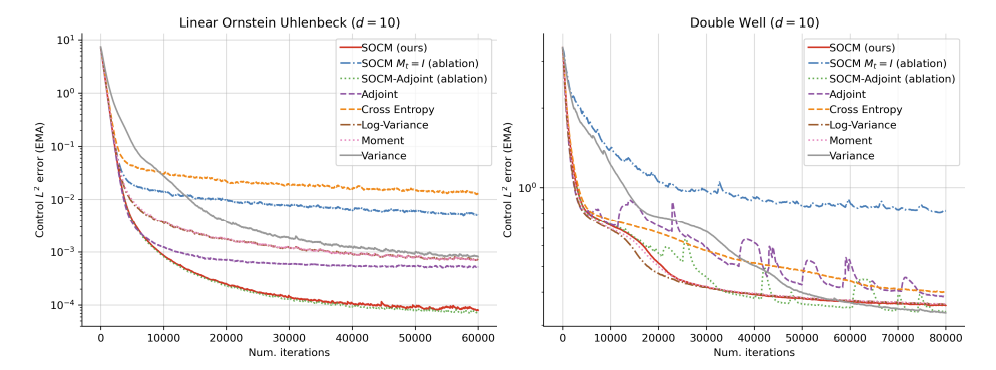
\includegraphics[width=0.95\textwidth]{figures/plots_1.png}
    \end{figure}
\end{frame}

\begin{frame}{Experimental Results (2/2)}
    \begin{figure}
        \centering
        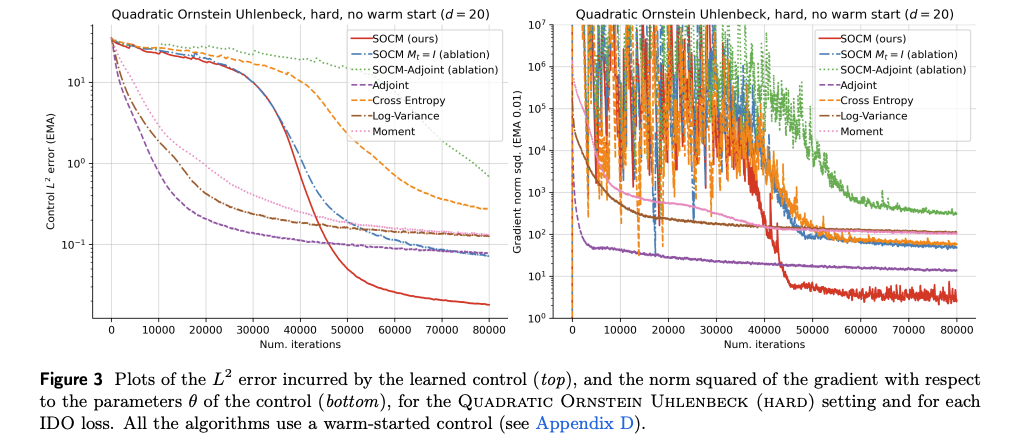
\includegraphics[width=0.95\textwidth]{figures/plots_2.png}
    \end{figure}
    \note{At the end of training, SOCM obtains the lowest L2
        error, improving over all existing methods by a factor of
        around ten. The two SOCM ablations come in second and third by a substantial difference, which underlines
        the importance of the path-wise reparameterization trick.
        \\
        \textcolor{red}{JE DOIS COMPRENDRE CE QUE EST UN ORNSTEIN UHLENBECK PROCESS}
        }
\end{frame}

%------------------------------------------------

%------------------------------------------------
\section{Conclusion}

\begin{frame}{Conclusion}
    \begin{block}{Paper's conclusion}
    peepee
    \end{block}

    \begin{alertblock}{Personal thoughts}
    poopoo
    \end{alertblock}

    \note{The main roadblock when we try to apply SOCM to more challenging problems is that the variance of the
        factor alpha(v, Xv, B) explodes when f and/or g are large, or when the dimension d is high. The control L2 error
        for the SOCM and cross-entropy losses remains high and fluctuates heavily due to the large variance of alpha
        The large variance of alpha is due to the mismatch between the probability measures induced by the learned
        control and the optimal control. Similar problems are encountered in out-of-distribution generalization for
        reinforcement learning, and some approaches may be carried over from that area (Munos et al., 2016).}
\end{frame}

%! so many links to do with RL and Monte Carlo Markov Chains which representent discretized differential equations
%------------------------------------------------

% \begin{frame}{Blocks of Highlighted Text}
%     In this slide, some important text will be \alert{highlighted} because it's important. Please, don't abuse it.

%     \begin{block}{Block}
%         Sample text
%     \end{block}

%     \begin{alertblock}{Alertblock}
%         Sample text in red box
%     \end{alertblock}

%     \begin{examples}
%         Sample text in green box. The title of the block is ``Examples".
%     \end{examples}
% \end{frame}


\begin{frame}{References}
    \footnotesize
    \bibliography{reference.bib}
    \bibliographystyle{apalike}
\end{frame}

%------------------------------------------------

\end{document}